\chapter{Planning and Task Clarification}
\label{ch:planning}

This chapter delves into planning and clarifying tasks for the prototype, as depicted in Figure \ref{fig:planning} following Pahl and Beitz's model. As mentioned previously in Chapter \ref{sec:methodicproductdevelopment}, this step plays a critical role in the product development process. They involve precisely defining and understanding the requirements and expectations related to a specific task or project. The goal is to eliminate confusion and ensure comprehension among all involved parties.

\begin{figure}[ht!]
    \centering
    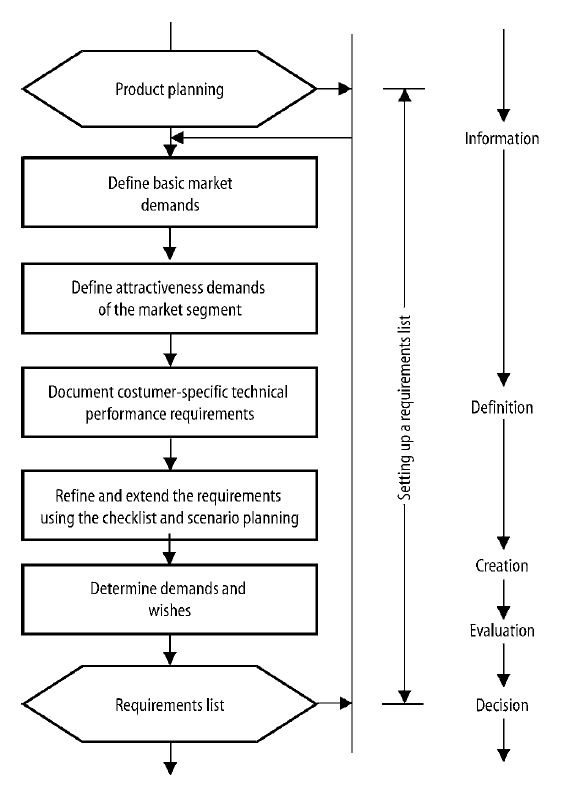
\includegraphics[width=0.6\textwidth]{texs/Part1/chapter2/image/planning.png}
    \caption{Planning and Task Clarification \cite{Pahl07m}}
    \label{fig:planning}
\end{figure}

During this step, the task's specific goals, limitations, and required deliverables are identified \cite{Pahl07a}. By clarifying and specifying tasks, engineers and designers set a strong foundation for the later stages of product development, which allows the designers to move forward with a clear sense of direction and focus. To achieve this, Pahl and Beitz formulated a series of questions that must be answered to ensure that the task is well-defined and understood \cite{Pahl07a}. These questions are:

\begin{itemize}
    \item What is the objective of the solution?
    \item What characteristics should the solution have?
    \item What characteristics should the solution avoid?
\end{itemize}

The requirements for the solution can be identified and spelled out by answering these questions. These requirements will serve as the basis for the subsequent phases of the product development process. The outcome of this step is a list of requirements that outline the needs, expectations, and restrictions tied to the task \cite{Pahl07a}.

\section{Establishing the Prototype's Requirements}
To properly establish the requirements for the prototype, it is suggested to properly define the objectives of the prototype and classify them into demands and wishes \cite{Pahl07n}.

Demands, as described by Pahl and Beitz \cite{Pahl07n}, are the essential and non-negotiable requirements that must be fulfilled for the product to be considered successful. They represent the core functionality and characteristics that the product must possess to meet its intended purpose and provide value to the users. Demands are typically based on objective criteria and are crucial for ensuring the product's functionality and compliance.

On the other hand, wishes, as defined by them, are desirable but non-essential requirements or features that clients or stakeholders would like to see in the product. Wishes often involve additional functionalities, aesthetics, or user experience enhancements that would provide added value or differentiate the product in the market. While wishes may not be mandatory, they can contribute to customer satisfaction, competitive advantage, and overall product excellence.

In addition, if possible, all of the requirements defined must be quantifiable, which means that the requirements must be measurable and testable \cite{Pahl07n}. This specification is essential for ensuring that the requirements are met and that the product can fulfill its intended purpose.


\section{Identifying the Prototype's Requirements}
In this section, the requirements of the prototype will be established. The checklist (see Figure \ref{fig:checklist}) will be used as a guideline to ensure that all the requirements are correctly identified and defined.

\begin{figure}[ht!]
    \centering
    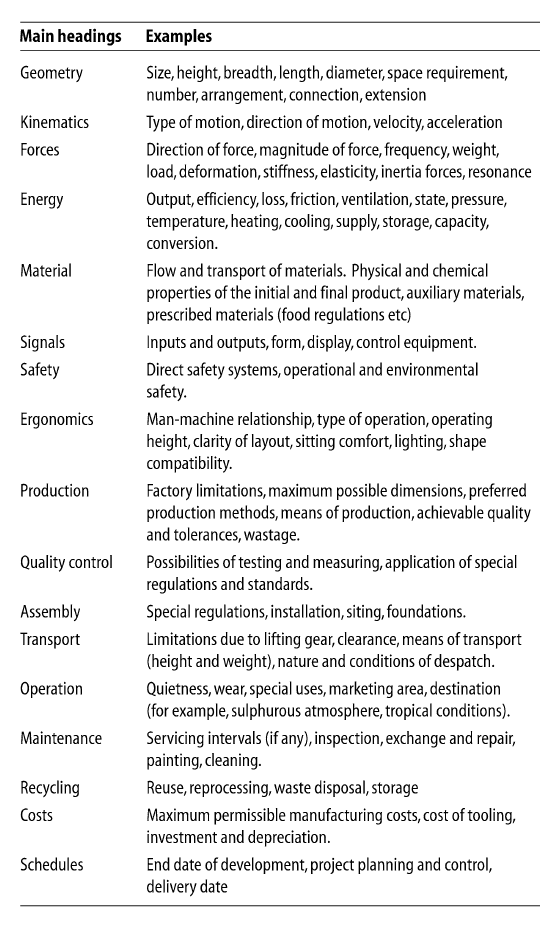
\includegraphics[width=0.6\textwidth]{texs/Part1/chapter2/image/requirements.png}
    \caption{Checklist for Establishing the Prototype's Requirements \cite{Pahl07o}}
    \label{fig:checklist}
\end{figure}

\subsubsection{Geometry}
When creating a prototype, adhering to specific size parameters is essential to ensure its functionality and usability for end-users or customers. The prototype must conform to a general size limit of 300 mm x 300 mm x 300 mm (length x width x height).

Additionally, we must consider the limitations of the 3D printer's size capacity. We have opted to employ the printer mentioned previously in Section \ref{subsec:prusa_slicer_mk3s}. This particular printer has a maximum printing area of 210 mm x 210 mm x 250 mm \cite{Prusa}.

Ideally, each printed component should fall within the specified printing size range. However, should a component exceed these dimensions, it will be necessary to divide it into two or more parts to facilitate printing. This approach guarantees that each part can be accommodated within the printer's size constraints.

\subsubsection{Energy}
The energy required for the prototype is crucial because it determines its usefulness and convenience. We have set a requirement that the prototype should function independently for at least an hour using the provided power supply. This guideline is in place to ensure that the prototype can function autonomously and provide users with a seamless experience.

By meeting this requirement, the prototype demonstrates that it can operate reasonably without frequent charging or relying on external power sources. This feature enables users to use the device without any concerns for an extended period, giving them more opportunities to explore its functionality and capabilities.

\subsubsection{Forces}
The force requirement for the prototype has two main aspects: ensuring it can handle the weight of its components while also adhering to a maximum weight limit.

Firstly, it is crucial to verify that the prototype can effectively support the weight of its components without compromising its overall structure or functionality, which ensures the prototype's durability and ability to withstand the forces exerted by its components. Additionally, it guarantees that the prototype can be manipulated and operated without the risk of damage or malfunction.

Furthermore, there is a specific constraint that the total weight of the prototype must not surpass 2 kg. This requirement encompasses the collective weight of all internal components, including predefined components and any additional materials integrated during the design process. Adhering to this weight limit ensures the prototype remains lightweight and manageable while meeting the intended performance criteria.

\subsubsection{Materials}
When developing the prototype, it is of utmost importance to thoughtfully consider the specific materials and elements that will be utilized. The client has already preselected specific components for this project, which are mandatory to meet the requirements. These components include the Raspberry Pi 4B, a 7-inch touch screen, and the Raspberry Pi Camera V2.

These elements are fundamental building blocks for the prototype's operation. The Raspberry Pi 4B, functioning as a versatile single-board computer, furnishes computational power and acts as the central control unit for the prototype. The 7-inch touchscreen enhances user interaction by providing a responsive and user-friendly interface for both input and output. The Raspberry Pi Camera V2 facilitates the capturing of images and videos.

\subsubsection{Ergonomics}
The prototype has specific ergonomics requirements regarding dimensions, weight, and handling. The main goal is to produce a compact and lightweight prototype, making it easy to carry and maneuver, which makes it more comfortable and convenient for users to handle.

Another crucial aspect of the ergonomics requirement is ensuring that users can comfortably hold the prototype. This requirement involves considering the prototype's shape, grip, and balance to ensure it is easy and secure. The design should fit naturally into the user's hand, providing a stable and ergonomic grip.

\subsubsection{Production}
The client has specified the fabrication of the prototype components to utilize the 3D Printing technology. Furthermore, the design of the prototype must accommodate the use of PLA filament. This material, known for its widespread availability and well-rounded combination of strength and flexibility, aligns with the requirements of the prototype.

\subsubsection{Operation}
The prototype must fulfill two essential requirements: easy to use freehand without additional support and compatible with a tripod to ensure stability.

The prototype design should allow freehand operation to achieve the first requirement. The design should be ergonomic, with a comfortable grip and easy-to-use controls, making it intuitive for users to use the prototype.

The second requirement is that the prototype should be able to integrate with a tripod to offer better stability when needed. This feature lets users securely attach the prototype to a tripod, ensuring a stationary and stable setup. With tripod compatibility, the prototype can cater to scenarios where steady and controlled operation or positioning is necessary.

\subsubsection{Assembly}
The assembly requirement for the prototype emphasizes the importance of considering the ease of assembly and disassembly of its components. This design consideration enables users to access the inner components easily, facilitating maintenance and repair tasks.

By designing the prototype with ease of assembly in mind, it becomes simpler for users to put the components together without requiring complex tools or specialized knowledge. This requirement promotes user-friendliness and reduces the time and effort required for initial assembly or subsequent modifications. Similarly, easy disassembly allows users to access the internal components when needed, simplifying troubleshooting, repairs, or component replacements.

The prototype's design should have swappable properties so individual components or modules can be easily removed and replaced without disassembling the entire prototype. Swappable parts enhance modularity, flexibility, and cost-effectiveness, as users can upgrade or replace specific components as needed rather than replace the entire prototype.

\subsubsection{Costs}
The cost requirement for the prototype focuses on the total cost of production. The manufacturing of the prototype must be within a budget of 300 €, excluding the cost of the predefined components. This budget encompasses the cost of all materials and components used in the production process.

\subsubsection{Schedules}
The schedule requirement for the prototype focuses on the time required for the design and production phase. The prototype's design must allow for manufacturing within a 2-month window, covering the entire production process, from design to assembly.

\subsubsection{Durability}
The durability standard for the prototype encompasses considerations for its ability to withstand dust and water, if possible. While achieving complete resistance may only sometimes be attainable, efforts should be directed toward enhancing the prototype's durability in these aspects.

Concerning dust resistance, the prototype's design should minimize the entry of dust particles into its internal components and sensitive areas. This requirement entails using appropriate seals, filters, or protective enclosures to prevent dust from negatively impacting the prototype's performance or functionality.

In terms of water resistance, if relevant to the intended use, the prototype should demonstrate a level of protection against water penetration. This specification may incorporate waterproof or water-resistant materials, seals, or coatings to shield the internal components from moisture.

\section{Requirement List}
Table \ref{tab:req1} and Table \ref{tab:req2} shows the list of requirements for the prototype, including the demands and wishes. The demands are marked with a D, while the wishes are marked with a W.

\begin{table}[H]
    \centering
    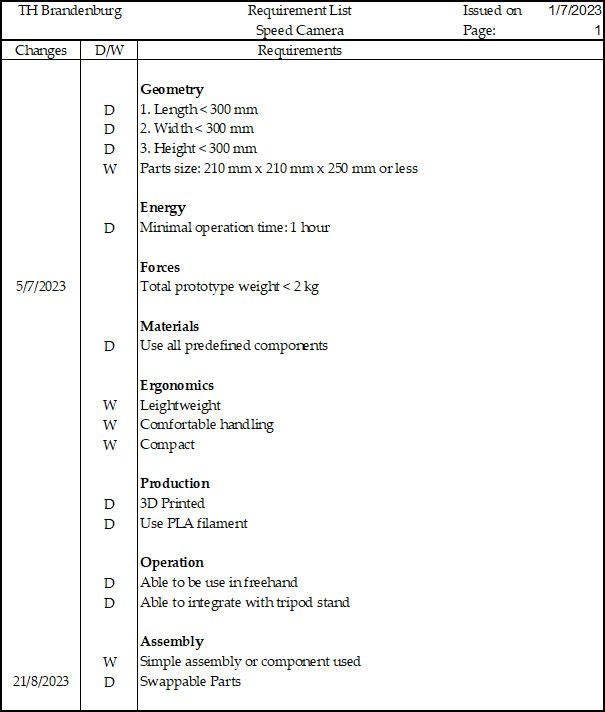
\includegraphics[width= 0.9\linewidth]{texs/Part1/chapter2/image/req1.png}
    \caption{Requirement List (1/2)}
    \label{tab:req1}
\end{table}

\begin{table}[H]
    \centering
    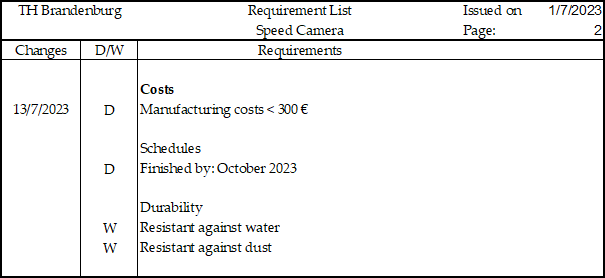
\includegraphics[width= 0.9\linewidth]{texs/Part1/chapter2/image/req2.png}
    \caption{Requirement List (2/2)}
    \label{tab:req2}
\end{table}
